\section{Logical View}
\label{section:logView}

In this section, the system will be described from a Mid-Level Design View, looking at the code itself.
Specifically, we will be looking at the variables and tools used to make the color changing of the triangle work.

\subsection{Mid-Level Design}

There are several key parts to the code that allow for triangle to be drawn each frame.

\subsubsection{Vertices}
The first key part is the vertices variable.
This variable is defined as an array with length 18.
I utilized 2 variables to help for changing the color later on in the code.

I utilized a variable colorValue to represent the value of the current color for the given vertex.
It is initialized to 1.0f to start with a colored triangle, similar to how the demonstration video starts.

Another variable I created was deltaColor which represents the rate of change for colorValue.
The use for this variable is explained later on in the render loop.

As seen in Figure \ref{Fig:vertices} below, the array is separated into 2 different sections: the positions of the points to generate the triangle, and the colors associated with that part of the triangle.
The ordering is x, y, z for the coordinates, eg. vertices[0] = 0.5f represents x = 0.5 on the cartesian coordinate system.
vertices[1] = -0.5f represents y = 0.5 also on the same plane.
Notice that there are no points lying outside of the cartesian plane since all z values = 0.
The colors represent RGB in order, thus vertices[3] = 1.0f represents the amount of red to apply.
vertices[4] and vertices[5] = 0.0f representing no values for Green and Blue respectively. 
Thus, the overall color of this vertex extending towards the other points of the triangle is red.

\begin{figure}[htb]
    \centering
    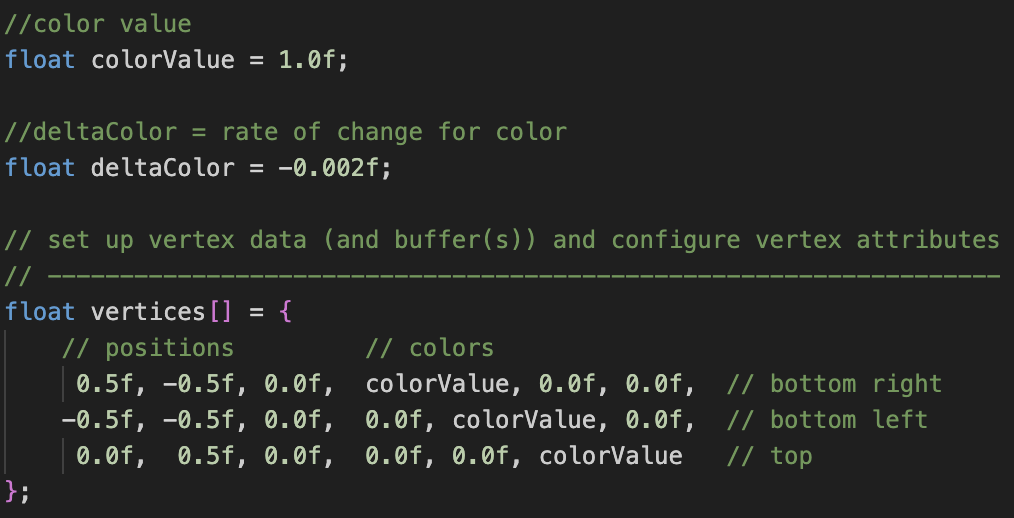
\includegraphics[width=10cm]{./Images/Vertices.png}
       \caption{Important Variables utilized for changing the color of the triangle.}
           \label{Fig:vertices}
\end{figure}

\newpage

\subsubsection{VBO and VAO}

Now having described the vertices variable in detail, I will briefly describe another set of key parts of the code: the VBO and VAO.

We use a VBO (Vertex Buffer Object) for managing the vertices variable.
The VBO is used for storing the vertex data, which in our case would be the position and color.
This is then sent to the GPU for fast rendering.

We also utilize a VAO (Vertex Array Object) for changing states of the VBO quickly and easily.
This proves useful for adjusting the state of the VBO from one color to the next in an efficient manner.

\subsubsection{Render Loop}

The final key part of the code is within the render loop.

The first portion worth mentioning is the function given which processes the user input.
This function allows for the user to close the program.

\begin{figure}[htb]
    \centering
    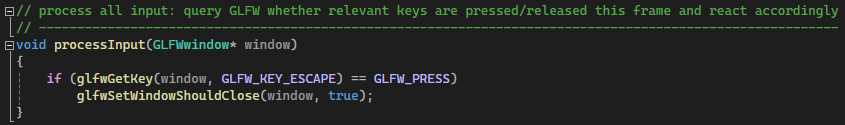
\includegraphics[width=10cm]{./Images/Escape.png}
       \caption{User Input logic.}
           \label{Fig:Escape}
\end{figure}

Another part of the render loop is the logic used to update the triangle.
This is done using the VAO and adjusting the previously mentioned variables colorValue and deltaColor.

\newpage

First, colorValue is added to deltaColor and subsequently set to the new value.
Then, the logic performs a boolean check to see if colorValue has hit or passed either extreme value for the color value possible for the system.
These values are 1.0 and 0.0 respectively.
If colorValue has reached either extrema or beyond them, then the sign of deltaColor is flipped.
This optimization allows for minimal code to be written and succinctly describing the process.

\begin{figure}[htb]
    \centering
    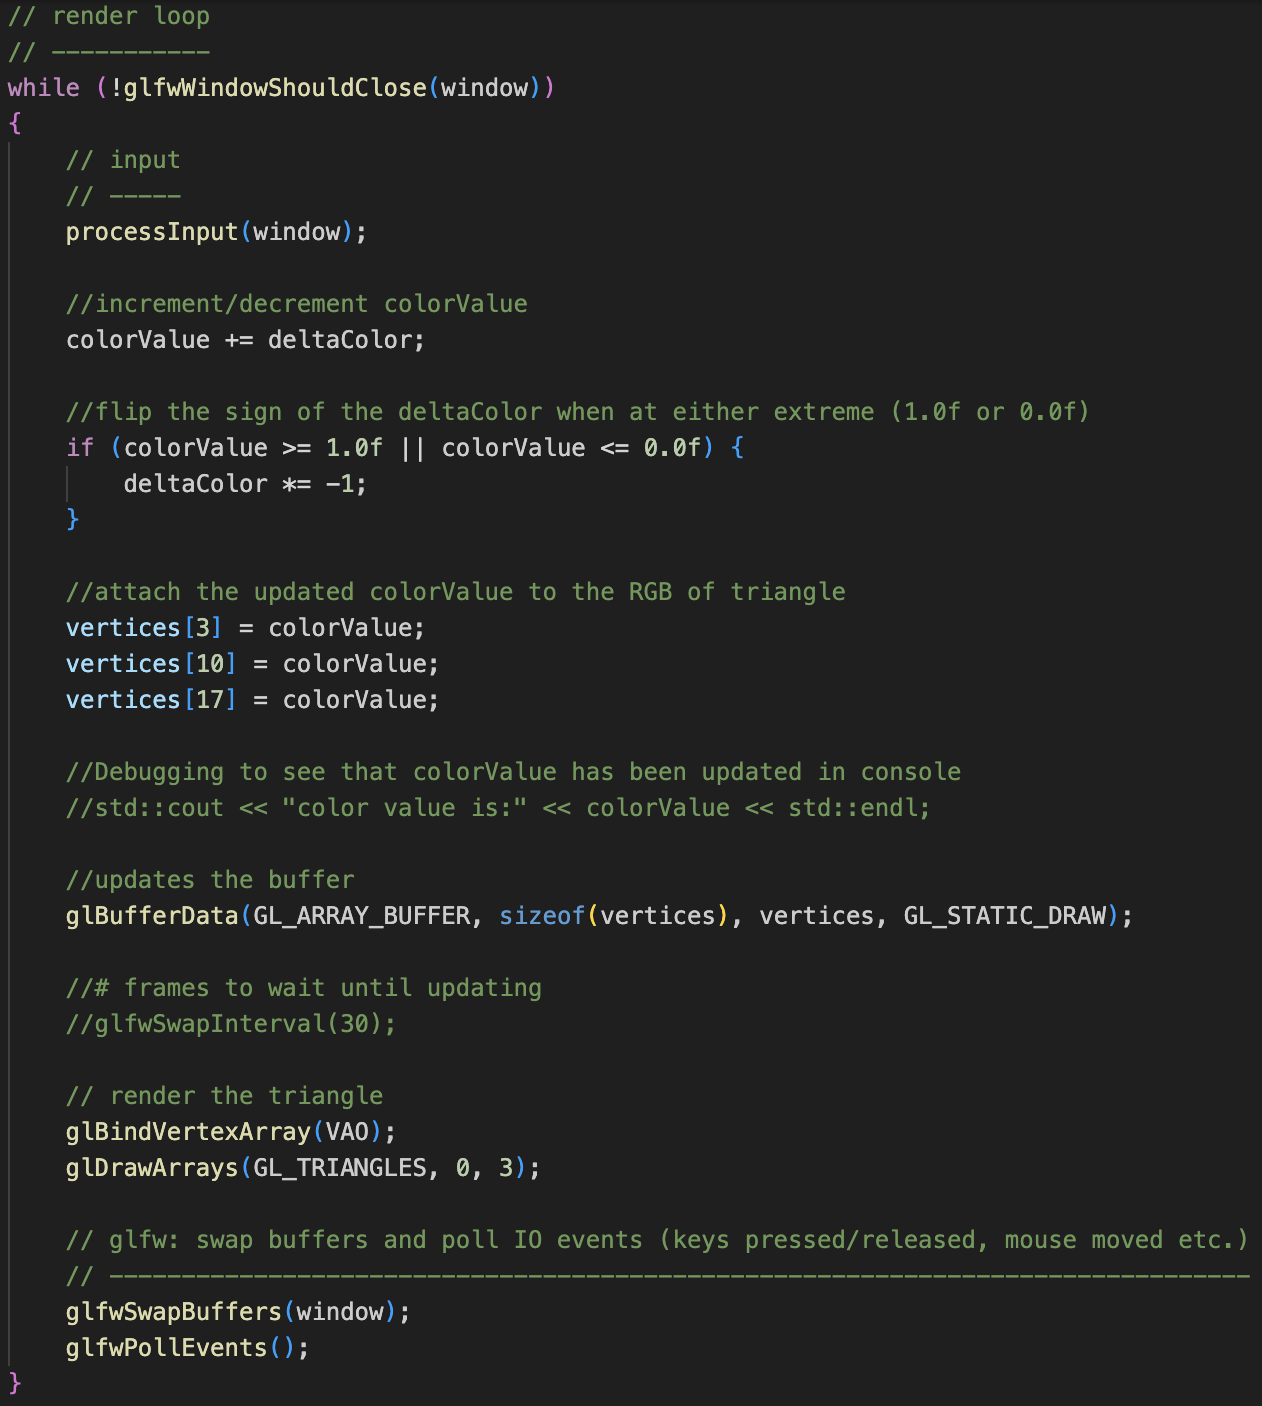
\includegraphics[width=10cm]{./Images/Render_Loop.png}
       \caption{Render Loop logic.}
           \label{Fig:renderloop}
\end{figure}

Afterwards, the newly updated colorValue is attached to the respective color value within the vertices variable.
Subsequently, we draw the buffer and utilize the VAO to render the triangle once again.

\newpage